\documentclass[pdftex,12pt,letter]{article}
\usepackage{fancyhdr}
\usepackage{enumerate}
\usepackage{tabularx}
\usepackage{graphicx}
\usepackage{array}
\usepackage[justification=justified,singlelinecheck=false]{caption}
\usepackage{placeins}
\pagestyle{fancy}
\makeatletter
  \renewcommand\@seccntformat[1]{\csname the#1\endcsname.\quad}
\makeatother

\newcolumntype {Y}{ >{\raggedright \arraybackslash }X}
\newcommand{\HRule}{\rule{\linewidth}{0.5mm}}
\captionsetup{labelformat=empty}

\begin{document}

\begin{titlepage}
\begin{flushright}
\HRule \\[0.4cm]
{ \bfseries
{\huge Inspection Report\\[1cm]}
{\large Reviewed by\\Jason Kuster, Stuart Long, and William Ordiway\\
\normalsize Moderated by Adrian Bubie}\\[1cm]
\normalsize Conducted at 11:33 pm on September 25th 2012}\\[1cm]
KOALAA Development\\[1cm]
October 1, 2012
\end{flushright}
\end{titlepage}
\begin{flushleft}
\section{Introduction}
\subsection{Purpose}
This inspection conducted by the KOALAA development team lists changes that should be made in the CWRUtility Software Requirements Specification version 1.0
\section{Inspection Action Log}

{\small 
\begin{tabular}{|r|c|l|p{6cm}|}
    \hline
Location & Severity & Type & Description \\
  \hline
  Title Page & Min & Typo & Ordiway is spelt wrong \\
    \hline
  Section 1.1 & Min & Typo & Solo is misspelled \\
   & Min & Typo & Correction is misspelled \\
   & Min & Redundancy  &  Delete "documented here are high priority" \\
  \hline
  Section 2.1 & Med & Rephrasing & Replace "encompassing 'all'" with 'most'\\
  \hline
  Section 2.2 & Min & Rephrasing & Change 'app' to 'applications'\\
    & Min & Typo & Delete duplicate 'is'\\
    & Min & Rephrasing & Change "installed users" to "people who have installed the application"\\
    & Min & Rephrasing & Change "the background" to "pulls data from each service"\\
\hline
	Section 2.3 & Min & Rephrasing & change 'shall' to 'will'\\
	\hline
	Section 2.5 & High & Change to Feature & Remove the tutorial feature\\
	\hline
Section 3.1.1 & Min & Typo & 'User' should not be capitalized\\
 & Min & Grammar & 'Service' should not be capitalized\\
\hline
Section 3.2.1 & Min & Tense & Change 'should be' to 'will be'\\
& Min & Grammar & "This" should have a noun after it\\
& Min & Grammar & Change 'but' to 'but also'\\
& Min & Grammar & Delete 'as well'\\
& Min & Aesthetics & Insert a line break at the end of the sentence\\
& High & Change to Feature & Removal of mapping navigation\\
& Med & Formatting & List a priority for this section\\
\hline
\end{tabular}
}
\newpage

\begin{tabular}{|r|c|l|p{6cm}|}
\hline
Section 3.2.2 & Mid & Formatting & Delete line breaks and change formatting so it is consistent with the rest of the document\\
 & High & Change to Feature & Delete Map.Navigate\\
\hline
Section 3.2.2 & Mid & Formatting & Delete line breaks, change formatting so it is consistent with the rest of the document\\
 & High & Change to Feature & Delete Map.Navigate\\
\hline
Section 3.3.1 & Very High & Redefined & Change the "NextBus" section to reflect that CRWRUtility will be implementing NextBus data into its UI and not simply embedding NextBus into the application\\
& Med & Formatting & List a priority for this section\\
& Min & Rephrasing & Change 'open application' to 'open feature'\\
& High & Change to Feature & Add 'select stop', 'route' and 'bus direction'  to functional requirements\\
\hline
Section 3.4.1 & Min & Rephrasing & Change 'location' to 'locations'\\
\hline
Section 3.4.3 & Min & Grammar & 'phone numbers' should be plural\\
& Min & Rephrase & Reword the Director.Call \\
\hline
Section 3.5.1 & Min & Rephrase & delete the 'of' in "will layout of the menus"\\
& Min & Typo & Change to "dinning hall"\\
& Min & Rephrasing & Change to "user selects a dinning hall to view"\\
& Med & Formatting & Deleted \textit{The Case Daily}\\
& High & Change to Feature & Change the priority of the 5YearCal to "lowest"\\
\hline
\end{tabular}
\end{flushleft}
\lfoot{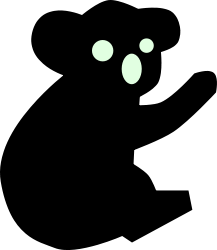
\includegraphics[height=1cm]{DarkKoala.png}}
\end{document}